\chapter{图形}

\section{基本图形}
相对于表格而言,LaTeX中的图形就简单多了,需要注意的是本模板推荐将所有图形都转化为pdf,具体内容参见图~\ref{fig_errorExpCH4}。
该图形放在本模板的本地文件夹figure中。
图~\ref{fig_errorExpCH4}是将Excel的五个子图形排布在一个ppt页面上,之后保存为pdf文件,最终得到的图形可以保证是矢量图。


\begin{figure}[htb]
  \centering
  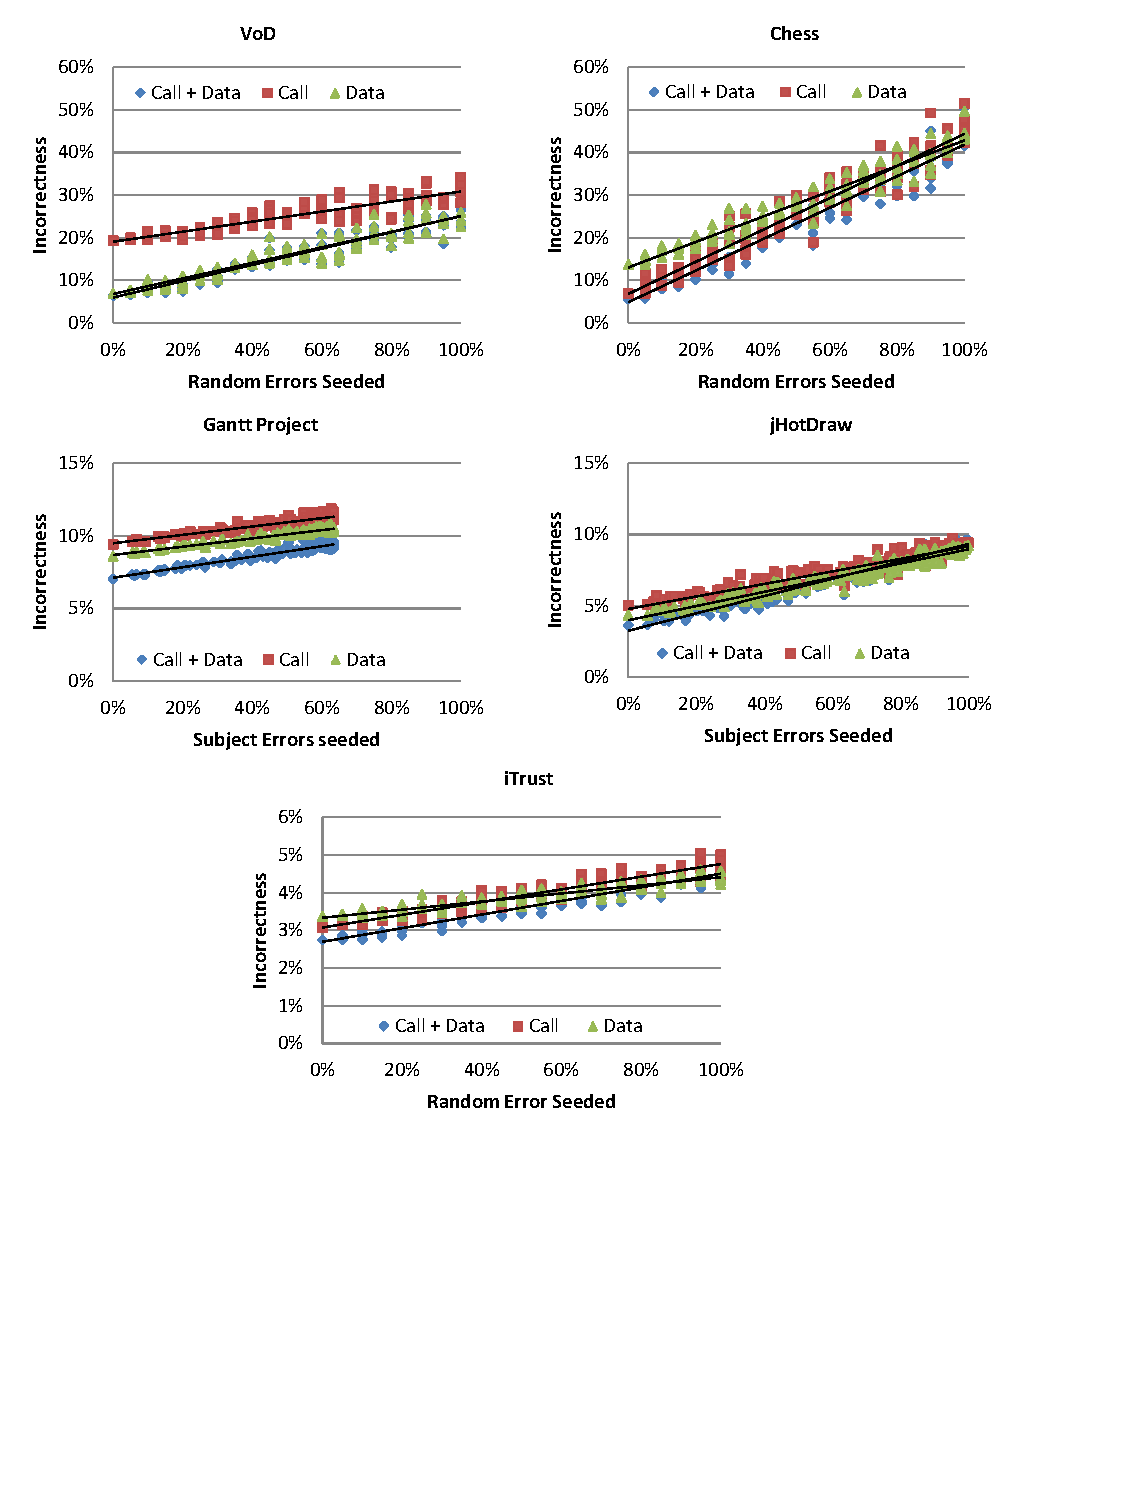
\includegraphics[width=5in]{figure/chapter4/errorExpCH4.pdf}
  \caption{以含错误的RTM为输入的五个系统上三个实验(Call,Data,Call+Data)的错误率(Incorrectness)}\label{fig_errorExpCH4}
\end{figure}

\textbf{注意:不要删除项目下面的njulogo、njuname和reviewPlaceholder这三个文件,分别是论文封面的校徽、手写体南大校名以及盲审时的空白占位符。}

\section{引用代码}

\begin{figure}[htb]
  \centering
  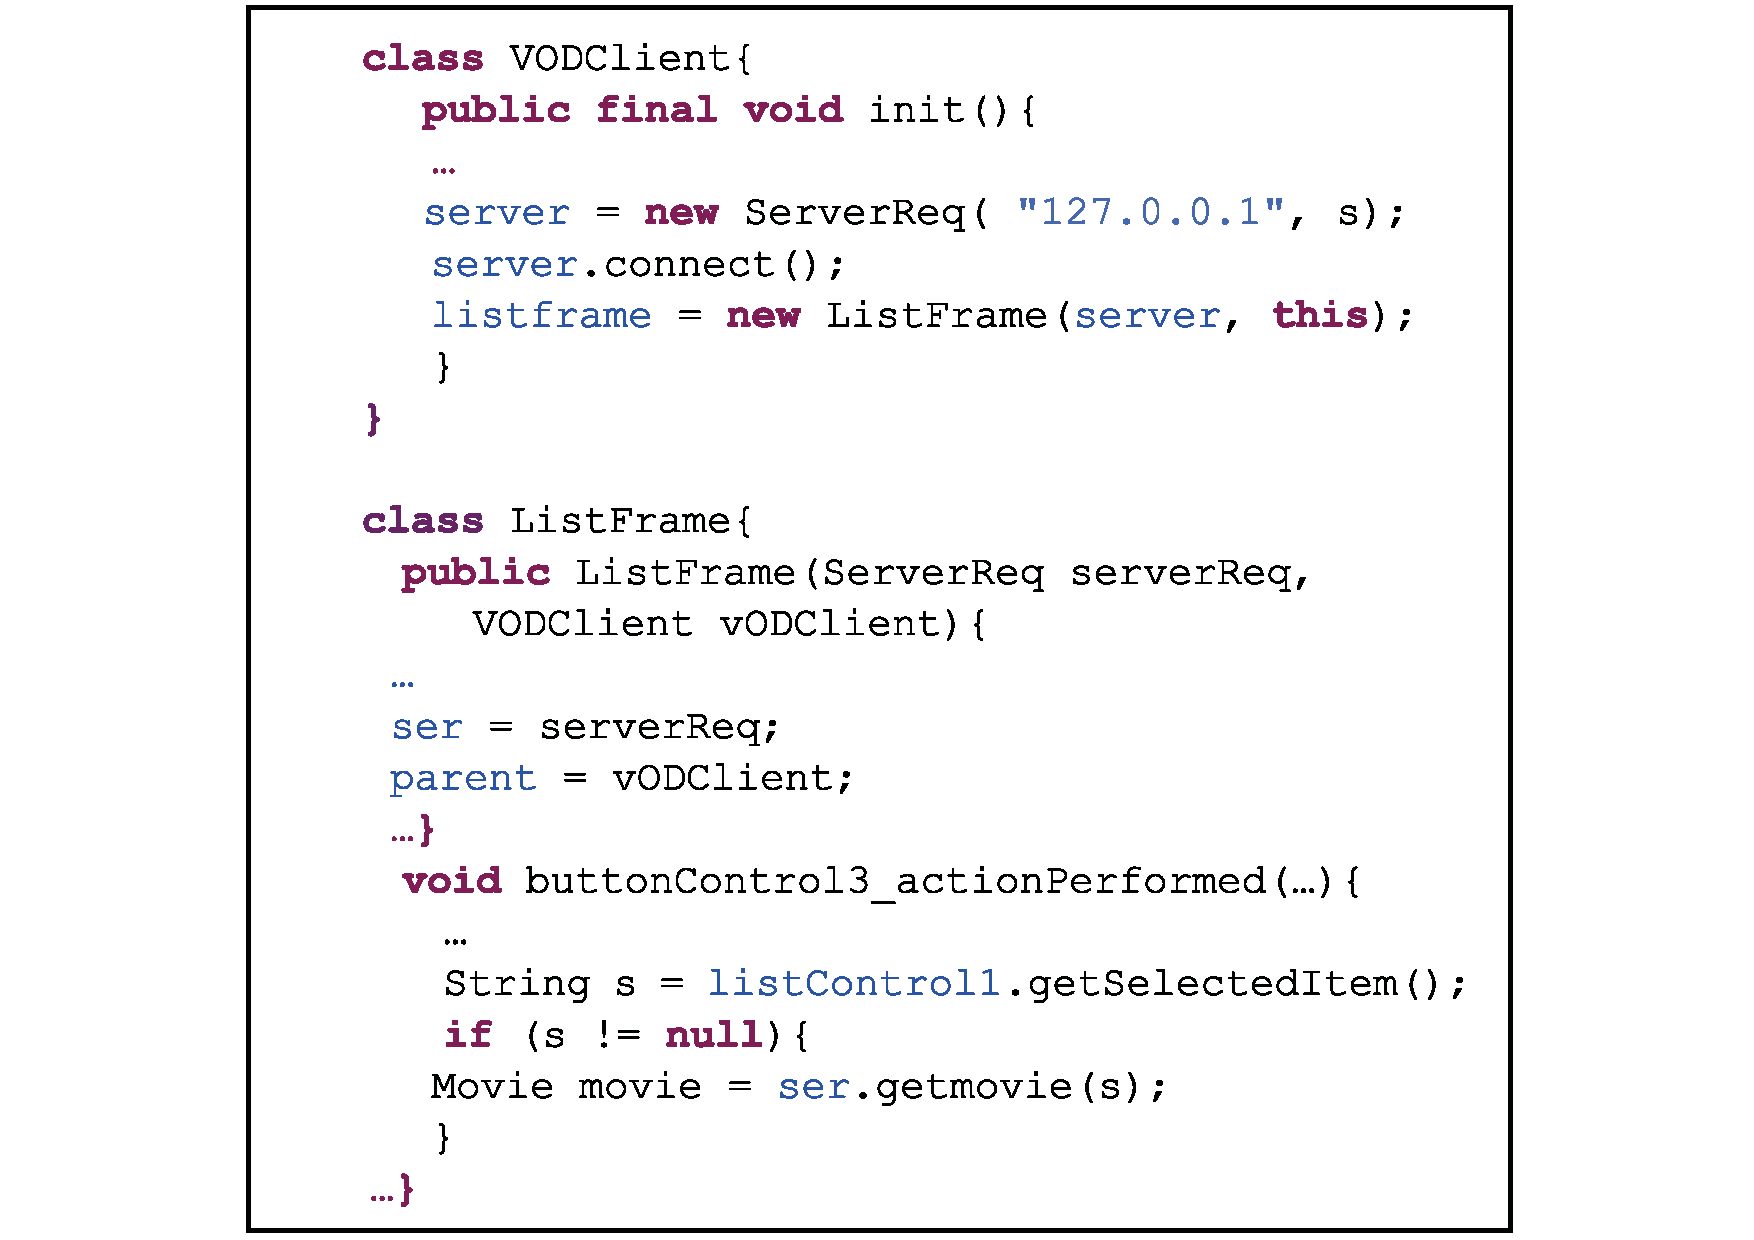
\includegraphics[width=\linewidth]{figure/chapter4/VoDCodeSample.pdf}
  \caption{VoD系统中的代码片段}\label{fig_VoDCodeSample}
\end{figure}

这里给出一个代码引用的推荐实践。
引用代码时先将代码放入word的文本框中,调整结束后,将该文本框页面另存为pdf文件,之后再作为图形来引用,如图~\ref{fig_VoDCodeSample}所示。

\section{其它图引用}

这里给出原模板提供的插图例子,请注意多行多图的设置方式。

一行一图,如图\ref{fig:line}。
\begin{figure}[htbp]
	\centering
	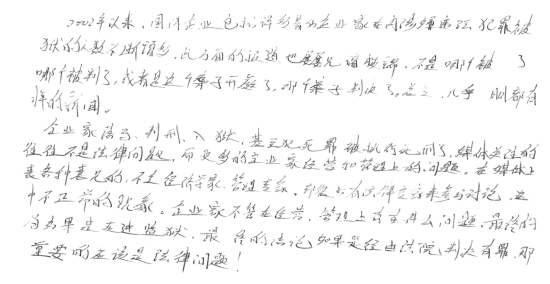
\includegraphics[width=0.7\textwidth]{figure/line.png} % requires the graphicx package
	\caption{待分行文本}
	\label{fig:line}
	%\vspace{0.8cm} % 用来调整和下方文字的间距
\end{figure}


一行两个图,如图\ref{fig:lstm}。
\begin{figure}[ht!]
	\centering
	\begin{subfigure}{.5\textwidth}
		\centering
		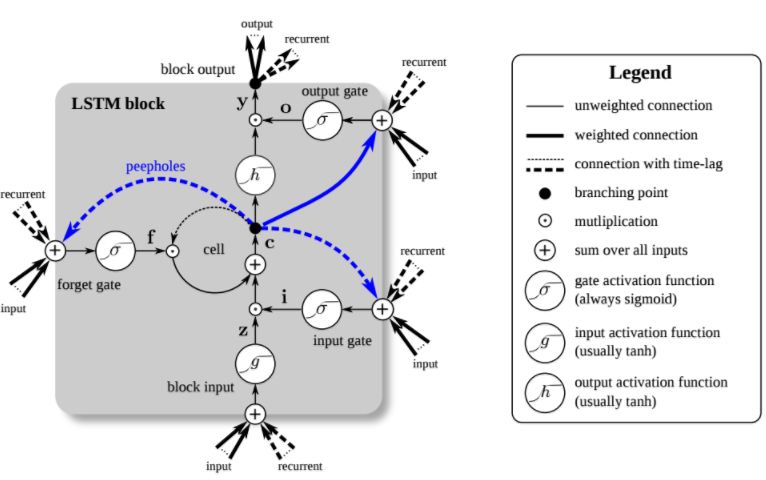
\includegraphics[width=0.9\textwidth]{figure/lstm1.png}
		\caption{长短时记忆单元模块}
	\end{subfigure}
	\begin{subfigure}{.4\textwidth}
		\centering
		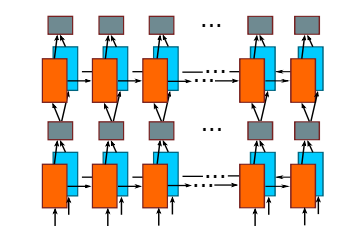
\includegraphics[width=0.8\textwidth]{figure/lstm2.png}
		\caption{深双向长短时记忆}
		\label{fig:lstm2}
	\end{subfigure}
	\caption{(a)一个长短时记忆单元模块。(b)深度双向长短时记忆的结构。}
	\label{fig:lstm}
\end{figure}

多行多图,如图\ref{fig:multi}。注意源文件中的双空行起到了子图换行的作用。
子图中大小不一是有意为之,请留意源码中subfigure和includegraphics后面的命令与四个子图大小之间的关系。

\textbf{注意:后续连续出现图形是最终文档中需要避免的情况,一般而言出现这种情况都是图贴的太多,文字写的太少导致的。建议针对每个图或表都采用“三段论”,即给出图表之前先介绍图表的大致情况与理由,然后给出图表,在图表展示之后再对图表中的内容进行讨论。}

\begin{figure}[ht!]
	\centering
	\begin{subfigure}{.69\textwidth}
		\centering
		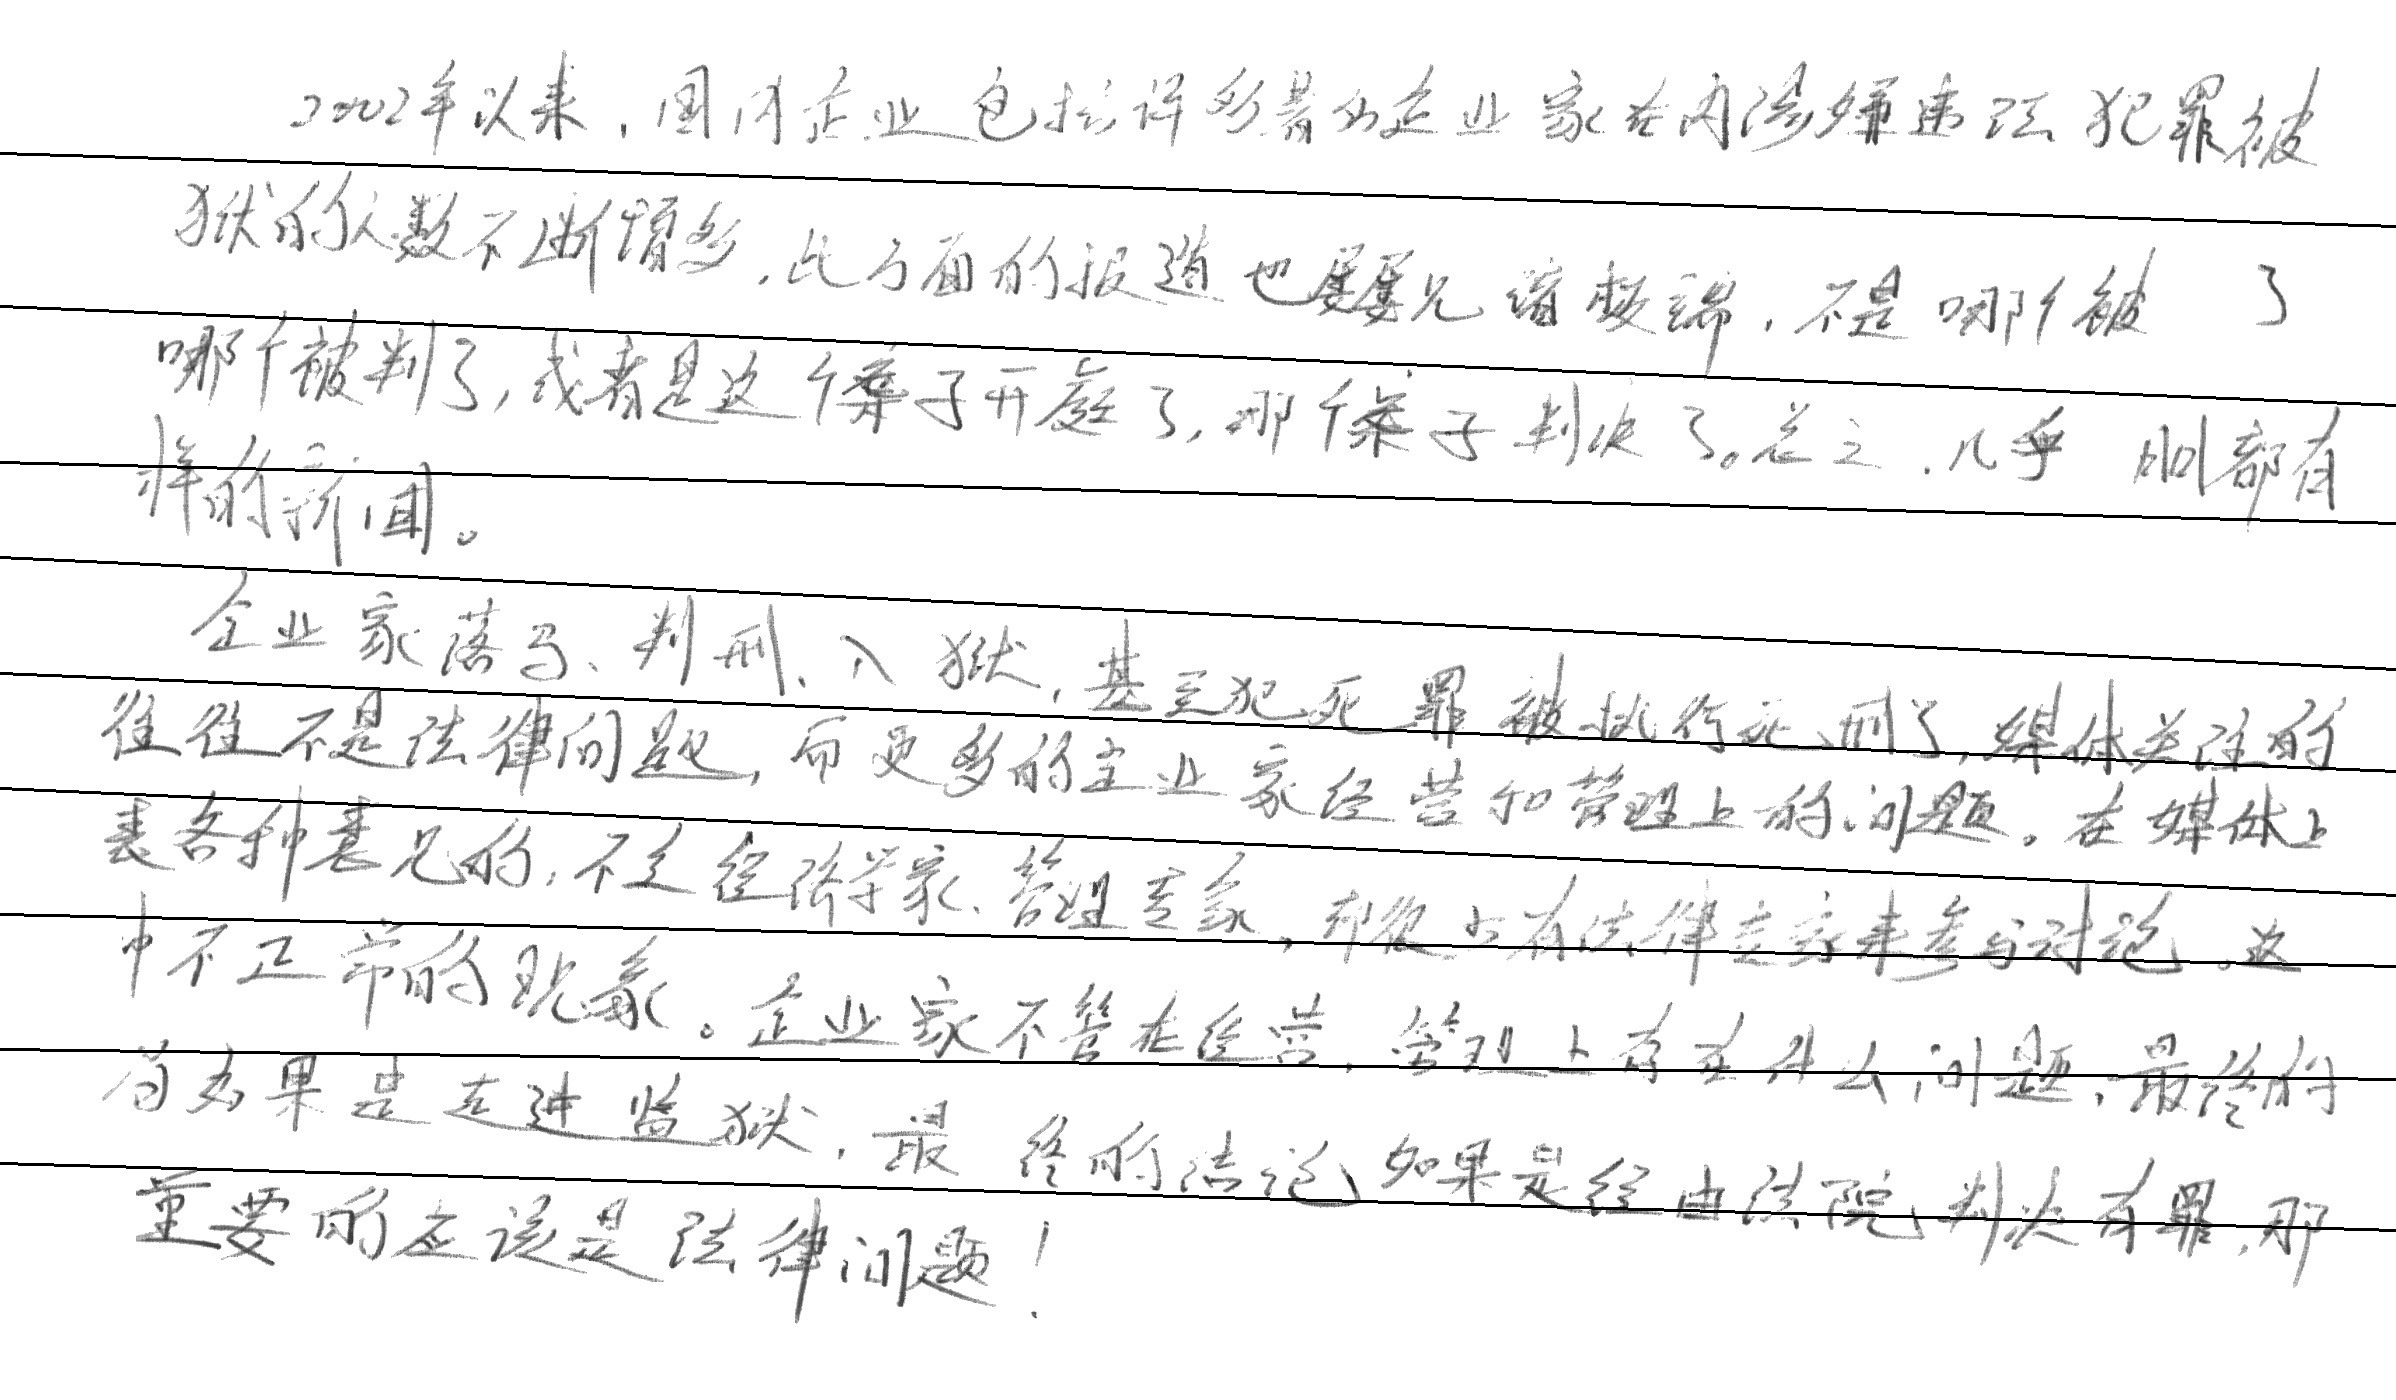
\includegraphics[width=1.0\textwidth]{figure/line1.png}
		\caption{全局损失切割第一行}
		\label{fig:line1}
	\end{subfigure}
	\begin{subfigure}{.3\textwidth}
		\centering
		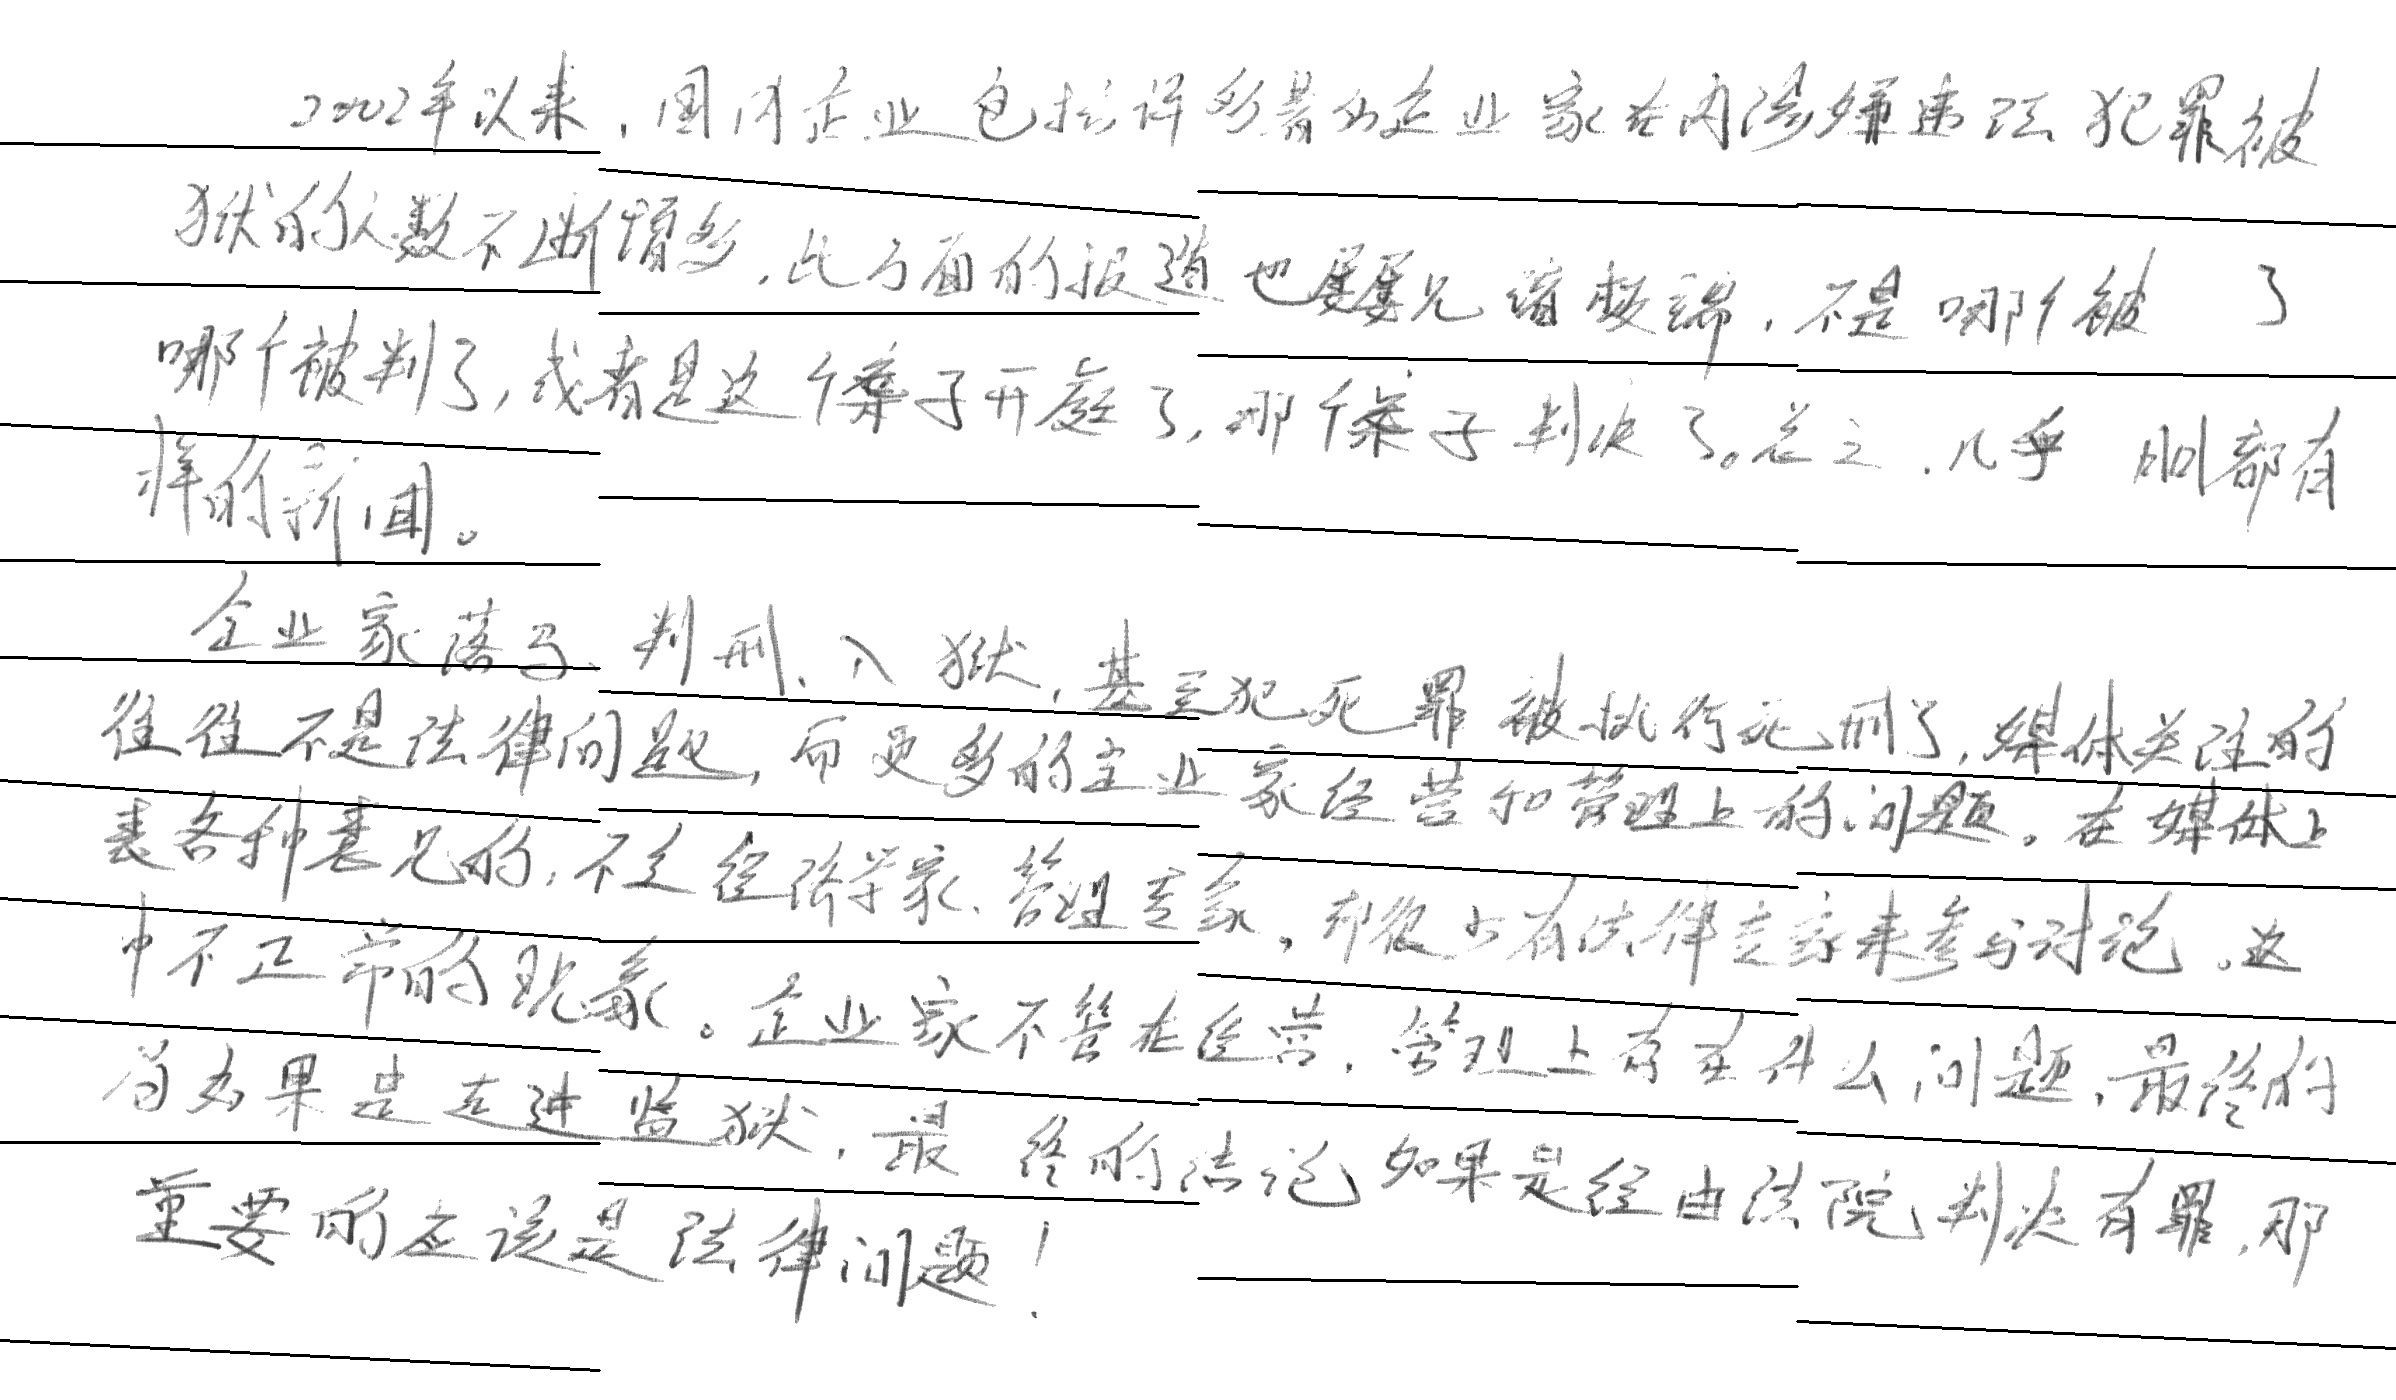
\includegraphics[width=1.0\textwidth]{figure/line2.png}
		\caption{局部损失切割第一行}
		\label{fig:line2}
	\end{subfigure}
	
	
	\begin{subfigure}{.49\textwidth}
		\centering
		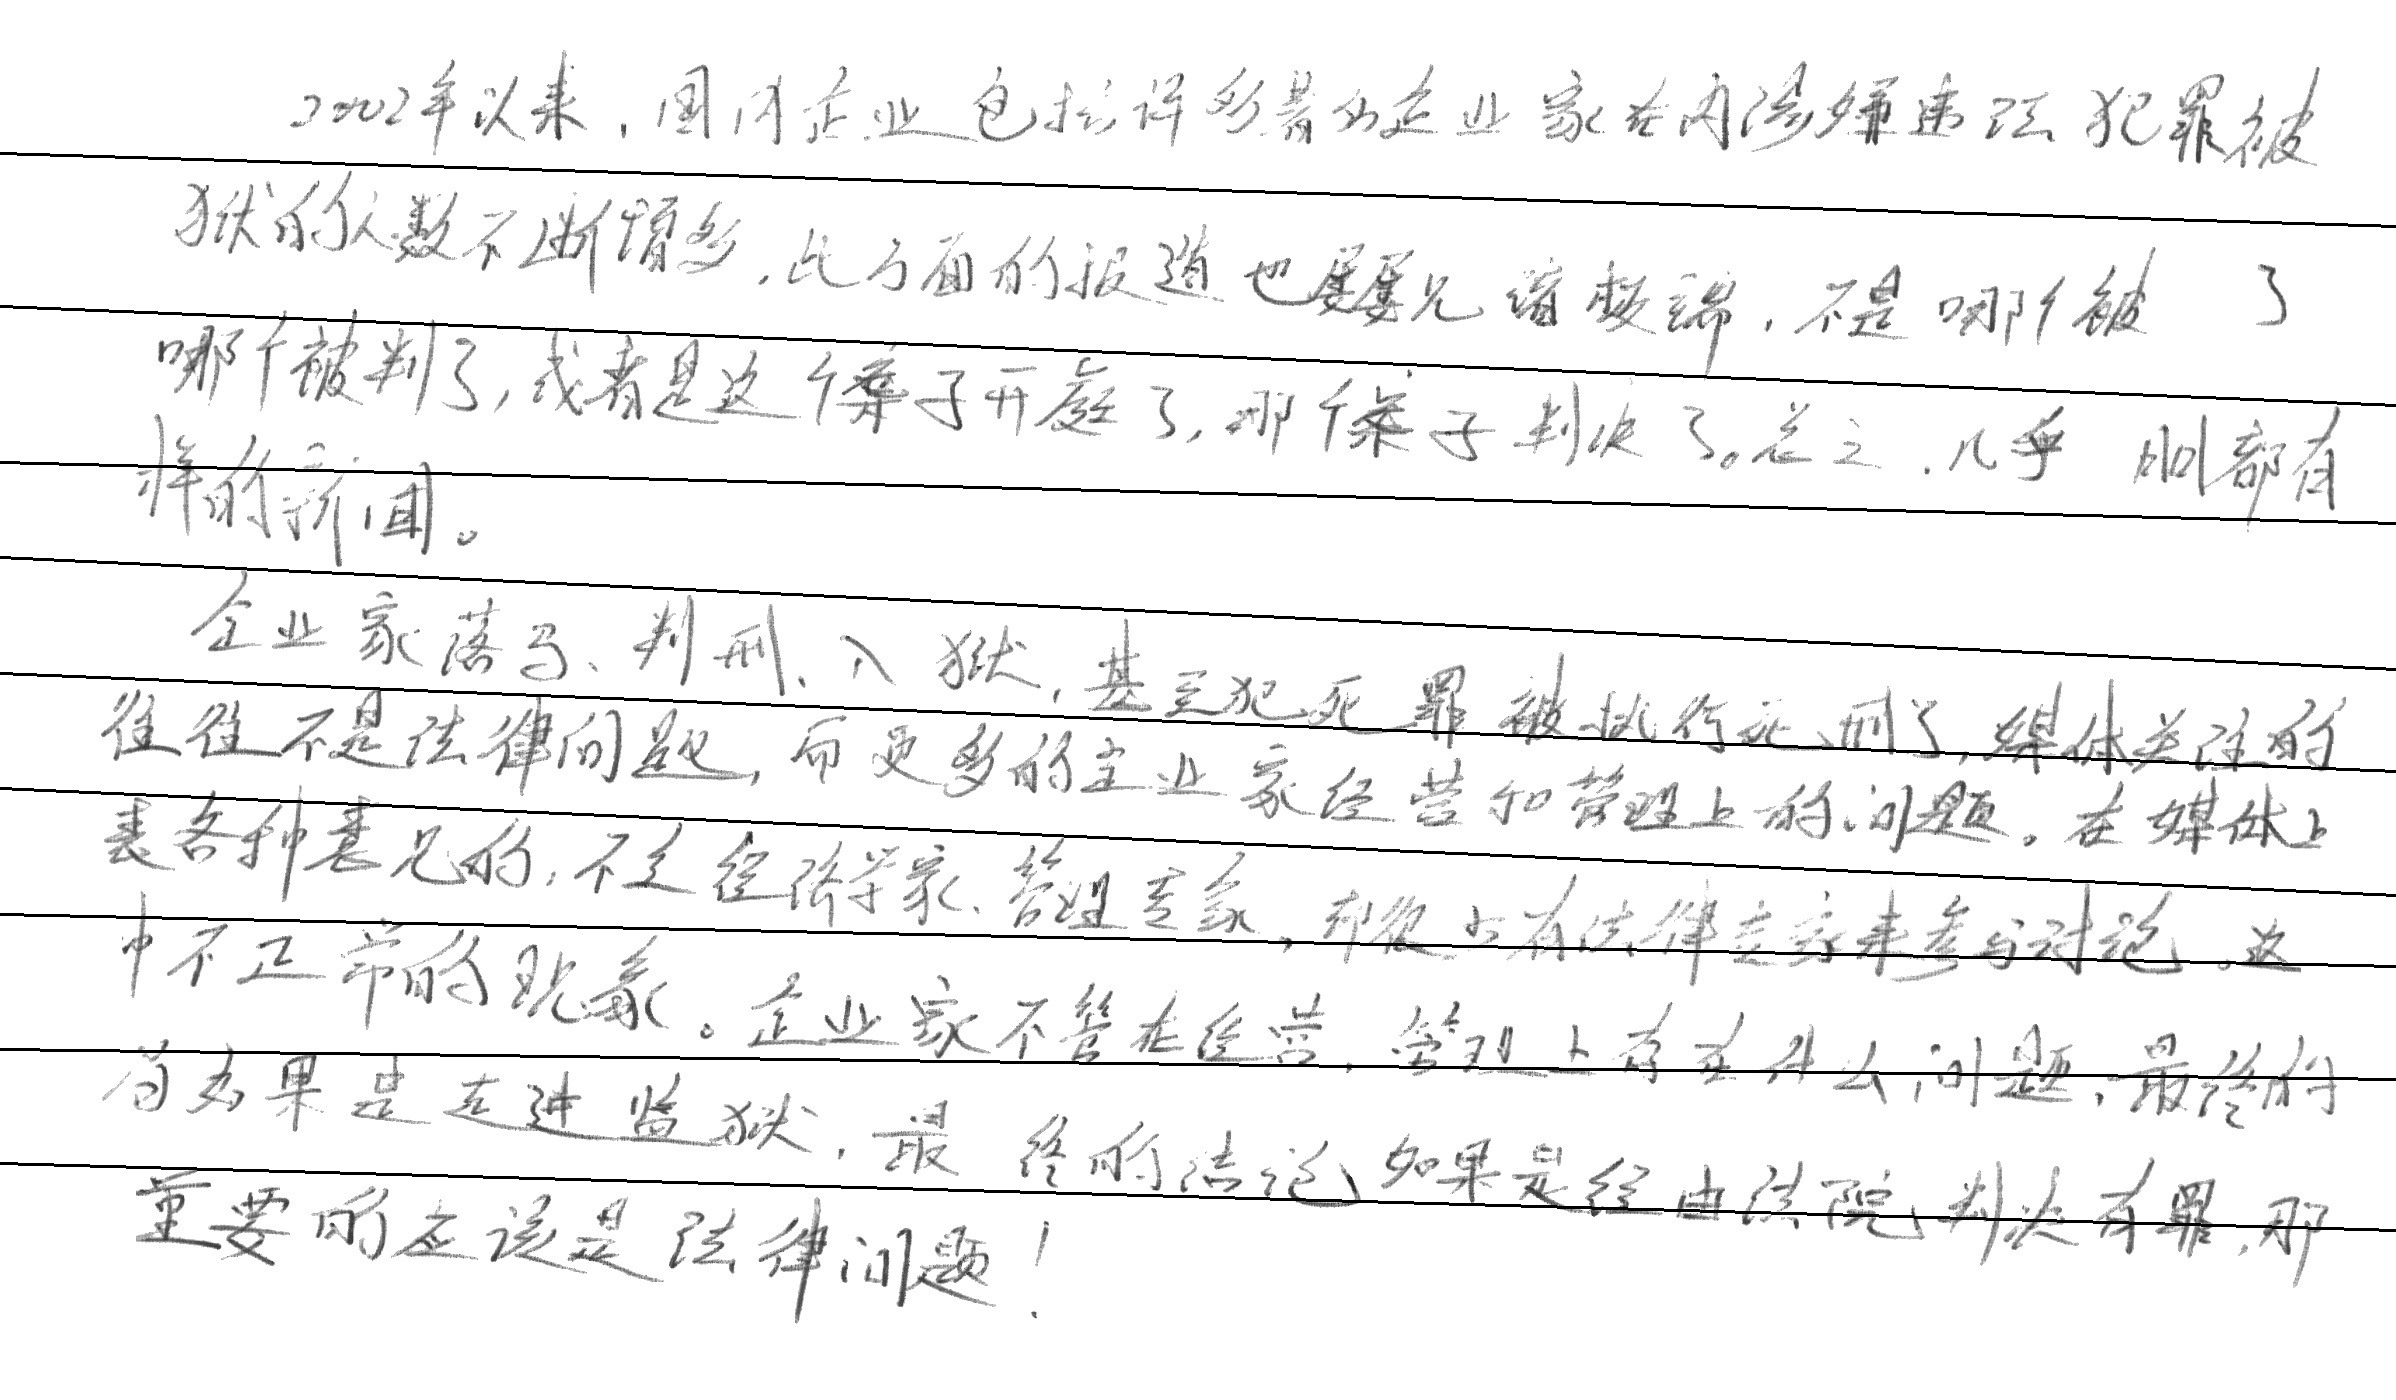
\includegraphics[width=0.5\textwidth]{figure/line1.png}
		\caption{全局损失切割第二行}
		\label{fig:line1}
	\end{subfigure}
	\begin{subfigure}{.49\textwidth}
		\centering
		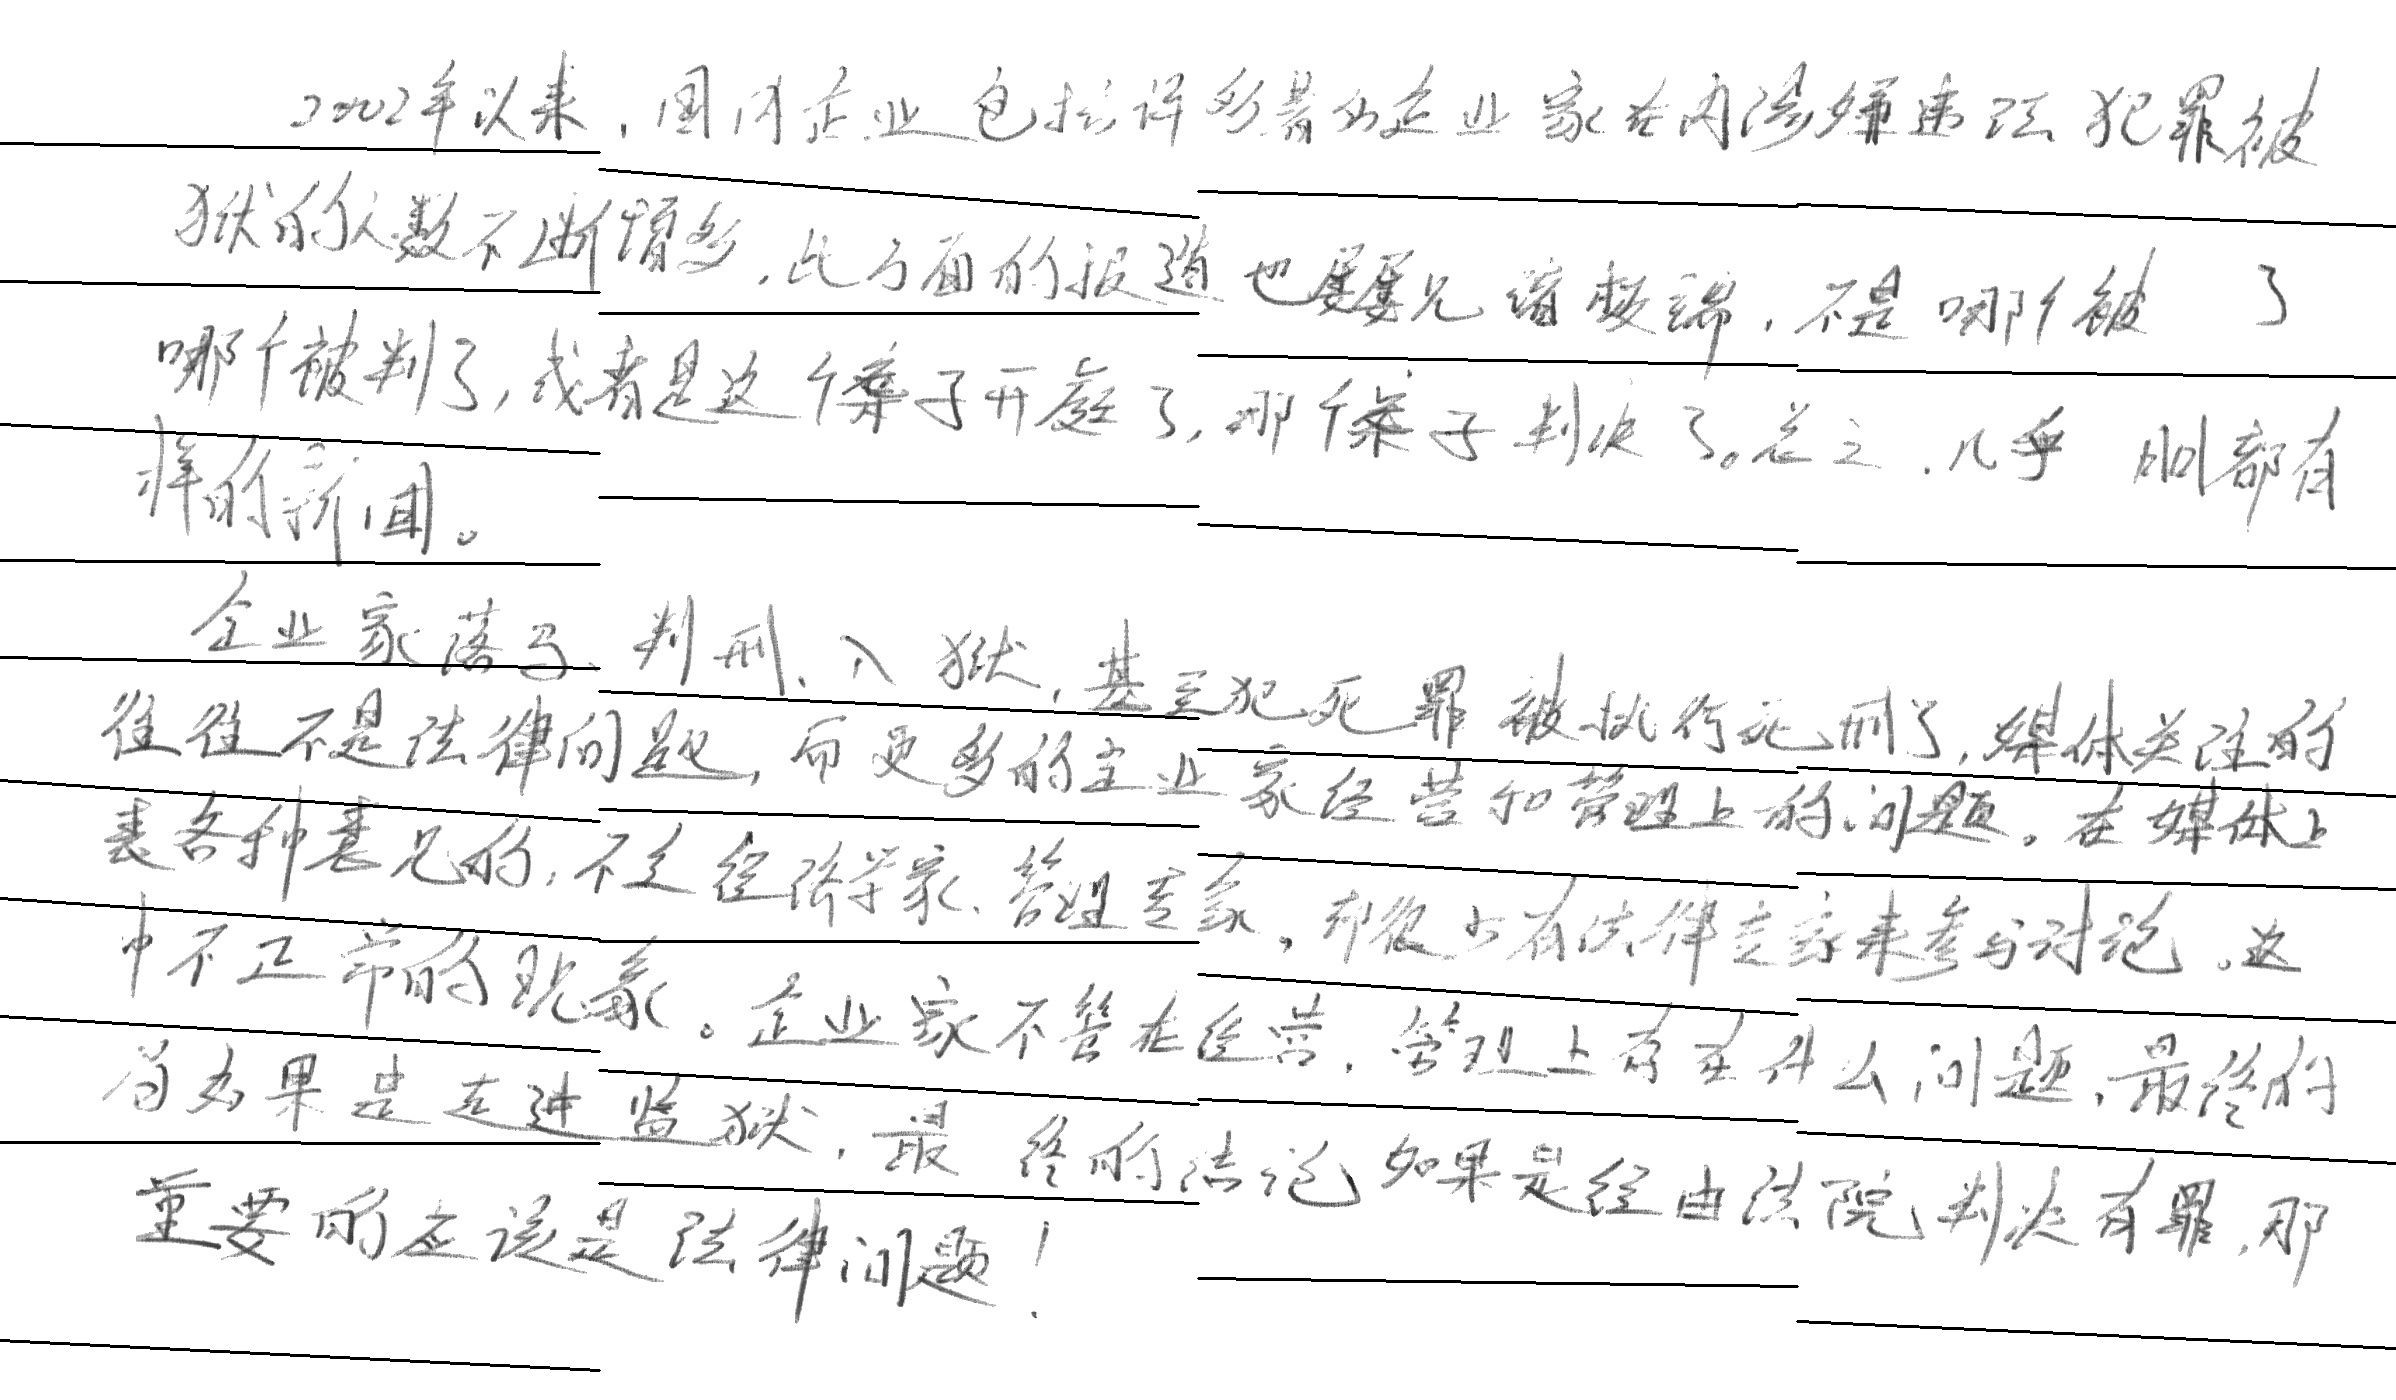
\includegraphics[width=0.8\textwidth]{figure/line2.png}
		\caption{局部损失切割第二行}
		\label{fig:line2}
	\end{subfigure}
	\caption{分行结果比较。(a)全局损失切割;(b)局部损失切割;(c)缩放的全局损失切割;(d)缩放的局部损失切割}
	\label{fig:multi}
\end{figure}

\newpage %为了将图片实例放在一起,另起一页,使用时请删掉


